\textbf{1-1.}一质点沿 $x$ 轴方向做直线运动, $t$ 时刻的坐标为 $x(t) = 5t^{2} - t^{3}$ , 式中 $x$ 以 $\mathrm{m}$ 为单位, $t$ 以 $\mathrm{s}$ 为单位。求: (1) 第 $3 \mathrm{~s}$ 至第 $4 \mathrm{~s}$ 内质点的位移和平均速度; (2) 第 $3 \mathrm{~s}$ 至第 $4 \mathrm{~s}$ 内质点所走过的路程。

\vfill

\textbf{1-2.}沿 $x$ 轴运动的质点, 其速度和时间的关系 $v(t) = t^2 + \pi \cos \frac{\pi}{6} t$ (SI 单位)。在 $t = 0$ 时, 质点的位置 $x_0 = -2 \mathrm{~m}$ 。试求: $t_1 = 3 \mathrm{~s}$ 时, (1) 质点的位置; (2) 质点的加速度。

\vfill
\newpage

\textbf{1-3.}一质点沿 $x$ 轴运动, 其加速度与位置的关系为 $a(x) = 2x + 4x^{2}$ (SI 单位), 已知质点在 $x = 0$ 处的速度为 $2 \mathrm{~m} / \mathrm{s}$ , 试求质点在 $x = 3 \mathrm{~m}$ 处的速度。

\vfill

\textbf{1-4.}一质点沿 $x$ 轴做直线运动, 其速度 $v$ 随时间 $t$ 的变化关系如习题1-4图所示。设 $t = 0$ 时, 质点位于坐标原点。试根据习题1-4图分别尽可能准确地画出,

(1) 表示质点运动的加速度 a 随时间 t 变化关系的 a-t 图;

(2) 表示质点运动的位移 $x$ 随时间 $t$ 变化关系的 $x - t$ 图。

\begin{figure}[H]
  \centering
  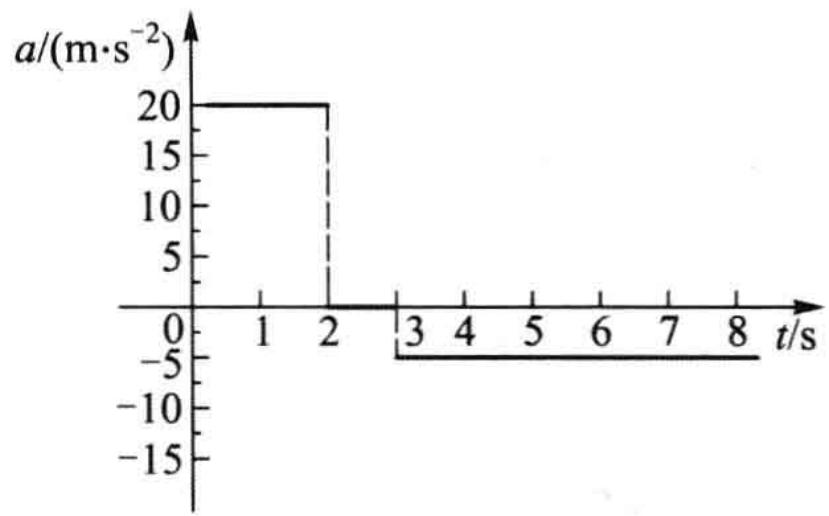
\includegraphics[width=0.4\textwidth]{figures/fig1-4.jpg}
\end{figure}

\vfill
\newpage

\textbf{1-5.}质点的运动学方程为 $r = 3ti + (2t^3 + 1)j$ (SI单位)。求：

(1) 自 $t_{0}=0$ 至 $t_{1}=1$ s 质点的位移；

(2) $t_{0} = 0$ 和 $t_1 = 1 \mathrm{~s}$ 两时刻质点的速度和加速度。

\vfill

\textbf{1-6.}一质点从 $r_0 = -5j$ m 位置开始运动, 其速度与时间的关系为 $v = 2ti + 5j$ , $r$ 以 $\mathrm{m}$ 为单位, $v$ 以 $\mathrm{m/s}$ 为单位。试问:

(1) 经过多少时间质点到达 x 轴?

(2) 此时质点位于 $x$ 轴上哪一点?

\vfill
\newpage

\textbf{1-7.}质点运动学方程为: $r = a \cos \omega t i + a \sin \omega t j + b t k$ , 其中 $a, b, \omega$ 均为正常量, 式中 $r$ 以 $\mathrm{m}$ 为单位, $t$ 以 $\mathrm{s}$ 为单位。

(1) 求质点速度和加速度与时间的关系式;

(2) 问质点做什么运动?

\vfill

\textbf{1-8.}离水面高度为 $h$ 的岸上有人用绳索拉船靠岸。人以恒定速率 $v_{0}$ 拉绳，求当船离岸的距离为 $s$ 时，船的速度和加速度。

\begin{figure}[H]
  \centering
  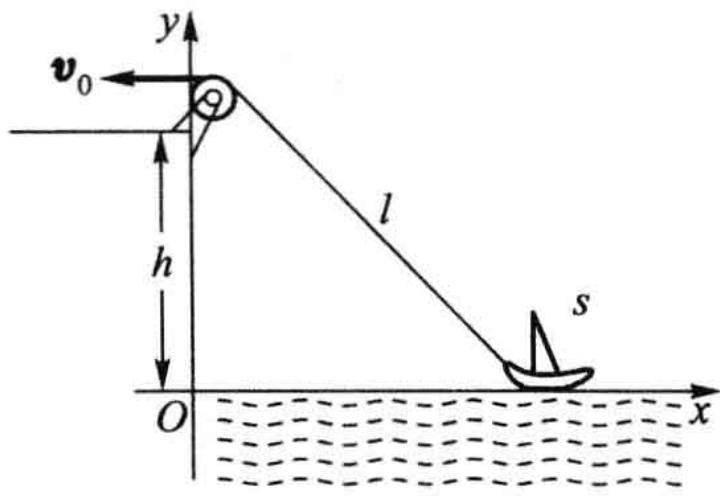
\includegraphics[width=0.3\textwidth]{figures/fig1-8.jpg}
  \end{figure}

\vfill
\newpage

\textbf{1-9.}如习题 1-9 图所示, 在桌面的一边, 一小球做斜抛运动。已知桌面高

$h = 1.0 \mathrm{~m}$ , 宽 $a = 2.0 \mathrm{~m}$ 。若欲使小球能从桌面的另一边切过, 并掉在离该边水平距离 $b = 0.50 \mathrm{~m}$ 处, 求小球的初速度 $v_{0}$ 和抛射角 $\theta$ 。

\begin{figure}[H]
  \centering
  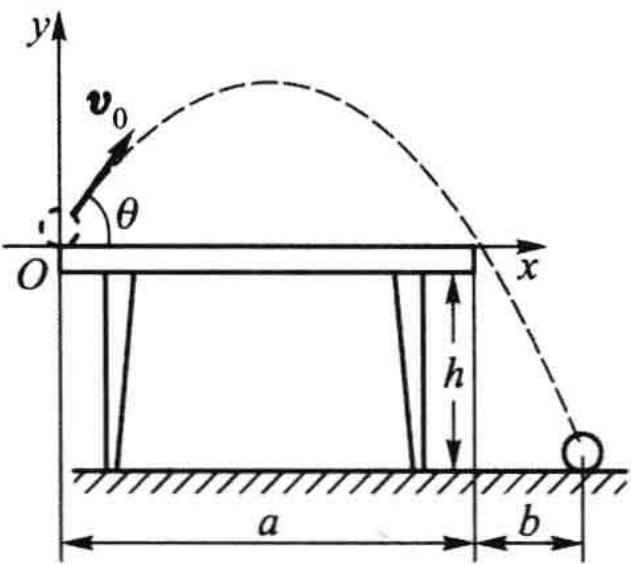
\includegraphics[width=0.3\textwidth]{figures/fig1-9.jpg}
  \end{figure}

\vfill

\textbf{1-10.}杆以匀角速 $\omega_0$ 绕过其固定端 $O$ 且垂直于杆的轴转动。在 $t = 0$ 时, 位于点 $O$ 的小珠从相对于杆静止开始沿杆做加速度为 $a_0$ 的匀加速运动。求小珠在 $t$ 时刻的速度和加速度。

\vfill
\newpage

\textbf{1-11.}有一半径为 $R$ 的定滑轮, 沿轮周绕着一根绳子, 悬在绳子一端的物体

按 $s = \frac{1}{2} bt^2$ 的规律向下运动, 如习题 1-11 图所示。若绳子与轮周间没有相对滑动, 试求轮周上一点 $A$ 在任一时刻 $t$ 的速度、切向加速度、法向加速度和总加速度大小。

\begin{figure}[H]
  \centering
  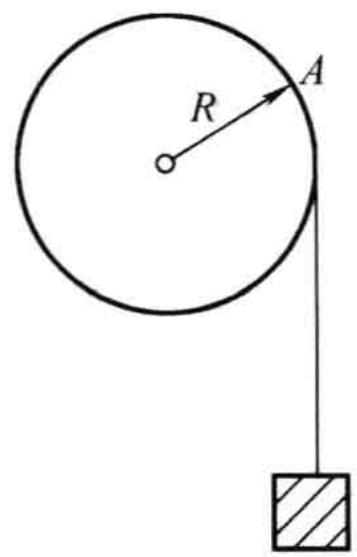
\includegraphics[width=0.2\textwidth]{figures/fig1-11.jpg}
  \end{figure}

\vfill

\textbf{1-12.}当蒸汽船以 $15 \mathrm{~km} / \mathrm{h}$ 的速度向正北方向航行时, 船上的人观察到船上的烟囱里冒出的烟飘向正东方向。过一会儿, 船以 $24 \mathrm{~km} / \mathrm{h}$ 的速度向正东方向航行, 船上的人则观察到烟飘向正西北方向。若在这两次航行期间风速不变, 求风速及方向。

\begin{figure}[H]
  \centering
  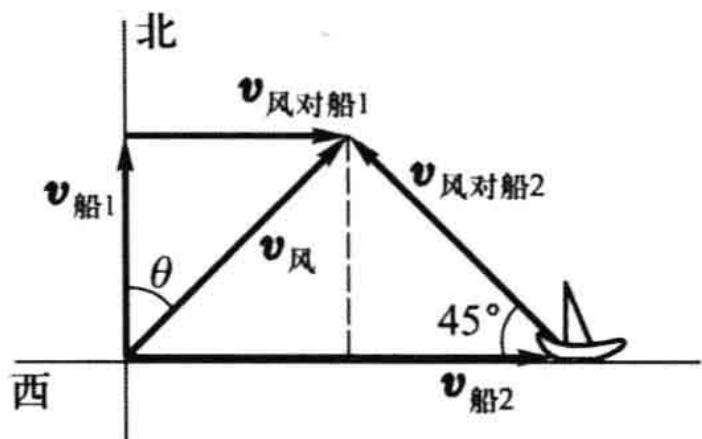
\includegraphics[width=0.3\textwidth]{figures/fig1-12.jpg}
  \end{figure}

\vfill
\newpage


\textbf{1-13.}一个自由落体在它运动的最后 $1 \mathrm{~s}$ 内所通过的路程等于全程的 $\frac{1}{3}$ 。求: (1) 物体下落的高度; (2) 通过全程所需的时间。

\vfill

\textbf{1-14.}一小球做竖直上抛运动,测得小球两次经过 $A$ 点和两次经过 $B$ 点的时间间隔分别为 $\Delta t_{A} 、 \Delta t_{B}$ ,如习题 1-14 图所示。求 $A 、 B$ 两点间的高度差 $h$ 。

\begin{figure}[H]
  \centering
  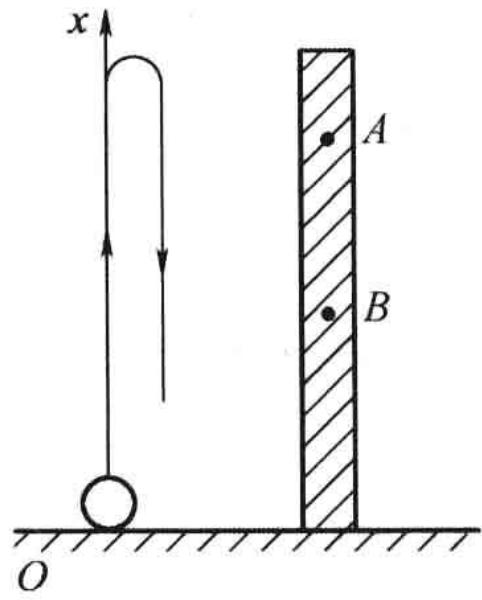
\includegraphics[width=0.25\textwidth]{figures/fig1-14.jpg}
  \end{figure}

\vfill
\newpage

\textbf{1-15.}汽车沿平直公路匀加速行驶,它通过某一段距离 $s$ 所需的时间为 $t_1$ , 而通过下一段相同距离 $s$ 所需的时间为 $t_2$ 。求汽车的加速度。

\vfill

\textbf{1-16.}火车从 A 城由静止开始沿平直轨道驶向 B 城, A、B 两城相距为 $s$ 。火车先以加速度 $a_{1}$ 做匀加速运动, 当速度达到 $v$ 后再匀速行驶一段时间, 然后刹车, 并以加速度大小为 $a_{2}$ 做匀减速行驶, 使之正好停在 B 城。求火车行驶的时间 $t$ 。

\vfill
\newpage

\textbf{1-17.}如习题 1-17 图所示, 物体从具有共同底边, 但倾角不同的若干光滑斜面顶端由静止开始自由滑下。问当倾角为何值时, 才能使物体滑至底端所需的时间最短?

\begin{figure}[H]
  \centering
  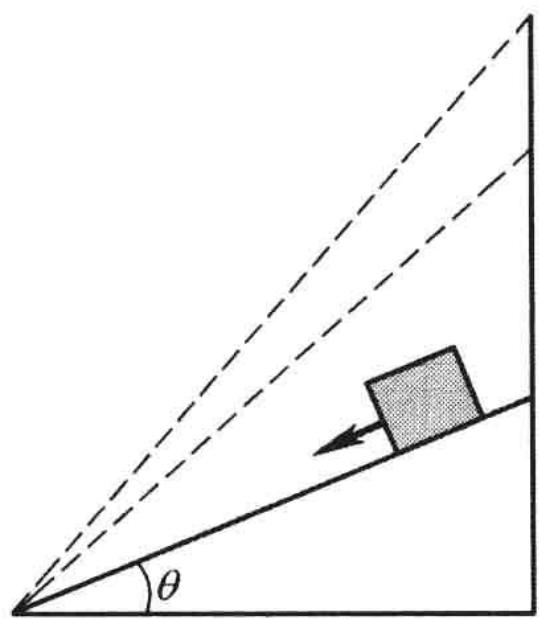
\includegraphics[width=0.25\textwidth]{figures/fig1-17.jpg}
  \end{figure}

\vfill

\textbf{1-18.}石块从楼顶以 $v_{0} = 10 \mathrm{~m} / \mathrm{s}$ 的速度被水平抛出, 落地时速度方向与水平方向之间成 $60^{\circ}$ 角, 求楼房的高度。

\vfill
\newpage

\textbf{1-19.}一物体被水平抛出,经过 $2.5 \mathrm{~s}$ 后,它的速度与加速度之间的夹角为 $45^{\circ}$ ,问又经过多少秒,它的速度与加速度之间的夹角变为 $30^{\circ}$ 。

\vfill

\textbf{1-20.}一小球从离地面高为 $h$ 的 $A$ 点处自由下落。当它下落了 $h_0$ 时, 与一斜面发生碰撞, 并以原速水平弹出, 如习题 1-20 图所示。问 $h_0$ 为多大时, 小球弹得最远?

\begin{figure}[H]
  \centering
  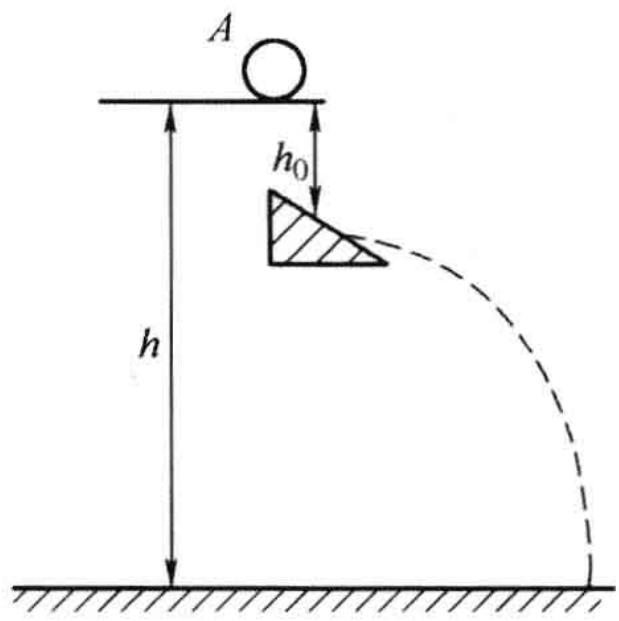
\includegraphics[width=0.3\textwidth]{figures/fig1-20.jpg}
  \end{figure}

\vfill
\newpage

\textbf{1-21.}斜向上抛出一物体,经过一段时间物体仍然向斜上方运动,此时速度方向与水平面成 $45^{\circ}$ 角,又过了相同的时间,物体已向斜下方运动,但速度方向与水平面仍成 $45^{\circ}$ 角。求物体的抛射角。

\vfill

\textbf{1-22.}在与水平面成 $\theta$ 角的山坡上, 一石块以 $v_{0}$ 的初速度做斜抛运动, 如习题 1-22 图所示。

(1) 若抛射角为 $\phi$ (抛出速度与水平面夹角), 求石块沿山坡方向的射程 $s$ ;

(2) 问抛射角 $\phi$ 为多大时, s 最大?

\begin{figure}[H]
  \centering
  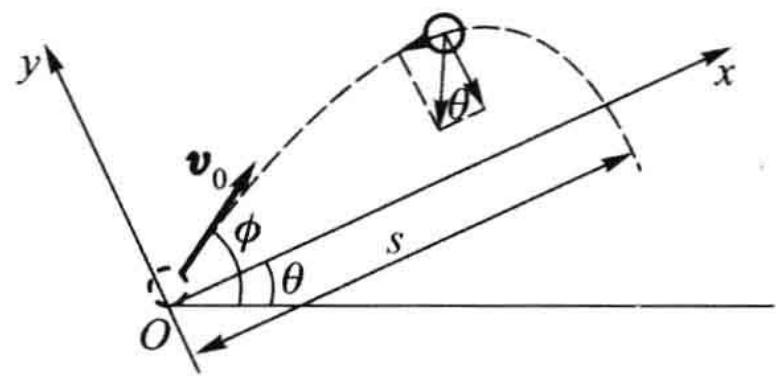
\includegraphics[width=0.4\textwidth]{figures/fig1-22.jpg}
  \end{figure}

\vfill
\newpage

\textbf{1-23.}从原点在竖直平面内以相同的初速度 $v_{0}$ 向各个方向投出许多质点。试证明：

(1) 任何时刻这些质点都处在同一圆周上;

(2) 它们的最高点位于同一椭圆上。

\vfill

\textbf{1-24.}汽车沿一圆周以 $v_{0} = 7.0 \mathrm{~m} / \mathrm{s}$ 的初速度匀减速行驶。经过 $t_{1} = 5 \mathrm{~s}$ 后，汽车的加速度与速度之间的夹角 $\theta_{1} = 135^{\circ}$ 。又经过 $t_{2} = 3 \mathrm{~s}$ 后，其加速度与速度之间的夹角 $\theta_{2} = 150^{\circ}$ 。求：

(1) 圆的半径 R;

(2) 切向加速度 $a_{\tau}$ ;

(3) 这两时刻的法向加速度 $a_{n1}$ 和 $a_{n2}$ 。

\begin{figure}[H]
  \centering
  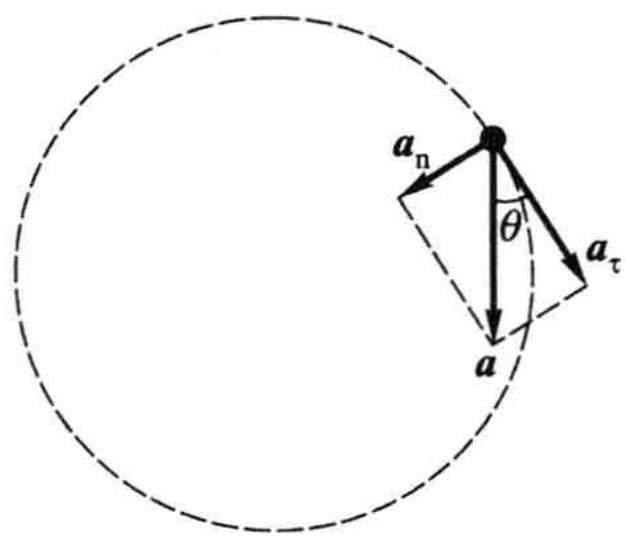
\includegraphics[width=0.3\textwidth]{figures/fig1-24.jpg}
  \end{figure}

\vfill
\newpage

\textbf{1-25.}一摩托车沿着半径 $R = 64 \mathrm{~m}$ 的圆周以 $v_{0} = 1 \mathrm{~m} / \mathrm{s}$ 的初速度行驶, 其切向加速度与时间的数值关系为 $a_{\tau} = \frac{1}{2 \sqrt{t + 1}}$ (SI 单位), 问 $t$ 为多少时, 总加速度最小?

\vfill

\textbf{1-26.}A 船以 $30 \mathrm{~km} / \mathrm{h}$ 的速度向东航行, B 船以 $45 \mathrm{~km} / \mathrm{h}$ 的速度向正北航行。求 A 船上的人观察到的 B 船的航速和航向。

\begin{figure}[H]
  \centering
  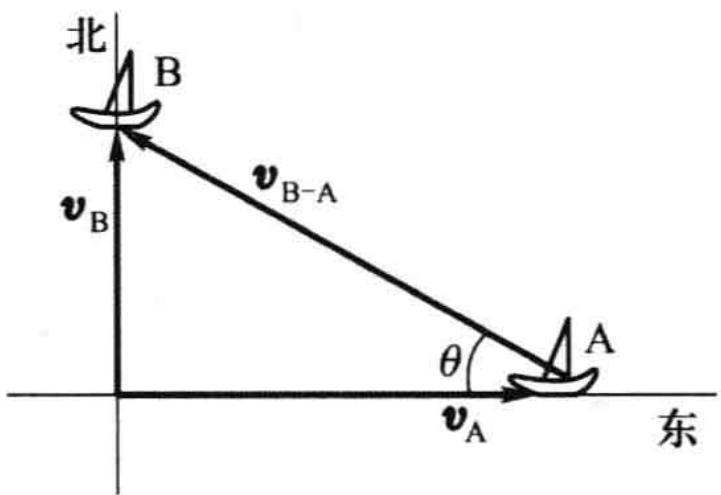
\includegraphics[width=0.4\textwidth]{figures/fig1-26.jpg}
  \end{figure}

\vfill
\newpage

\textbf{1-27.}一溜冰者在冰面上以 $v_{0} = 7 \mathrm{~m} / \mathrm{s}$ 的速度沿半径 $R = 35 \mathrm{~m}$ 的圆周溜冰。某时刻他平抛出一小球, 为使小球能击中冰面的圆心处, 他应以多大的相对于他的速度抛球? 并求出该速度的方向 (用与他溜冰速度之间的夹角 $\theta$ 表示)。已知人抛球时手的高度 $h = 1.5 \mathrm{~m}$ 。

\begin{figure}[H]
  \centering
  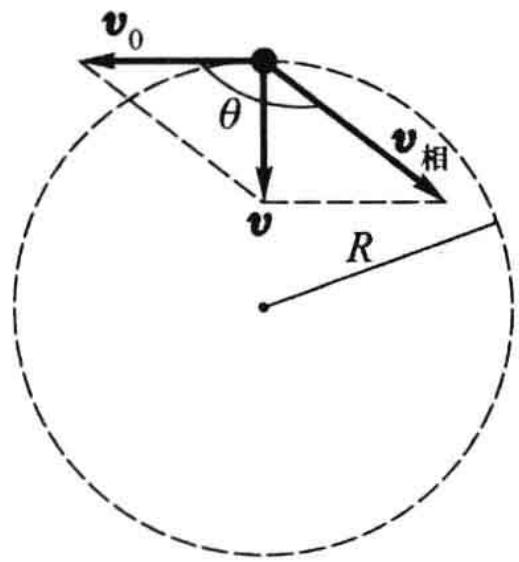
\includegraphics[width=0.25\textwidth]{figures/fig1-27.jpg}
  \end{figure}

\vfill

\textbf{1-28.}在宽为 $l$ 的河的两岸停着两艘小船, 它们的连线与河岸线成 $\alpha$ 角。已知两艘小船在静水中最大的划行速度分别为 $u_{1}$ 和 $u_{2}$ , 河水流速为 $v$ 。若它们同时出发, 则各应向什么方向划行才能在最短的时间内相遇? 并求出此时间。

\begin{figure}[H]
  \centering
  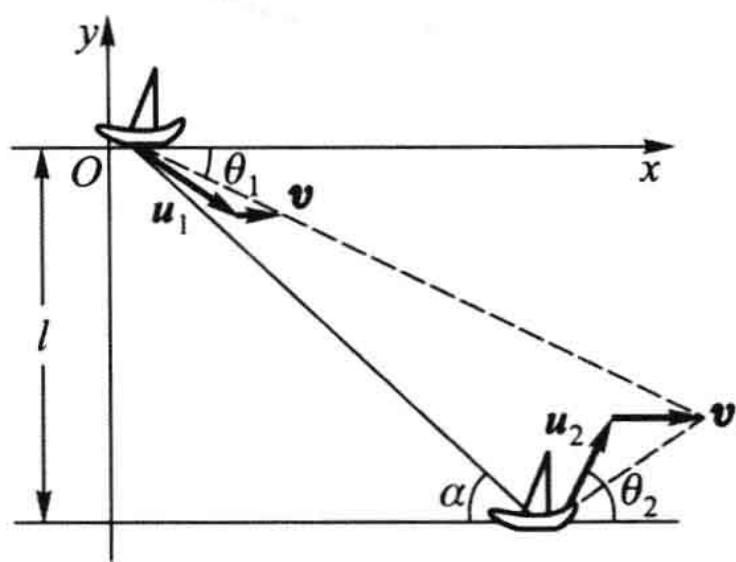
\includegraphics[width=0.3\textwidth]{figures/fig1-28.jpg}
  \end{figure}

\vfill
\newpage

\textbf{1-29.}一架飞机在无风时以匀速 $v$ 相对地面飞行, 能飞出的最远距离为 $R$ (包括飞出和飞回)。现在风速为 $u$ , 方向为北偏东、角度为 $\alpha$ 的风中飞行, 而飞行的实际航向为北偏东、角度为 $\beta$ 。求证: 在这种情况下, 飞机能飞出的最远距

$$
\frac {R \left(v ^ {2} - u ^ {2}\right)}{v \sqrt {v ^ {2} - u ^ {2} \sin^ {2} (\beta - \alpha)}}
$$

\begin{figure}[H]
  \centering
  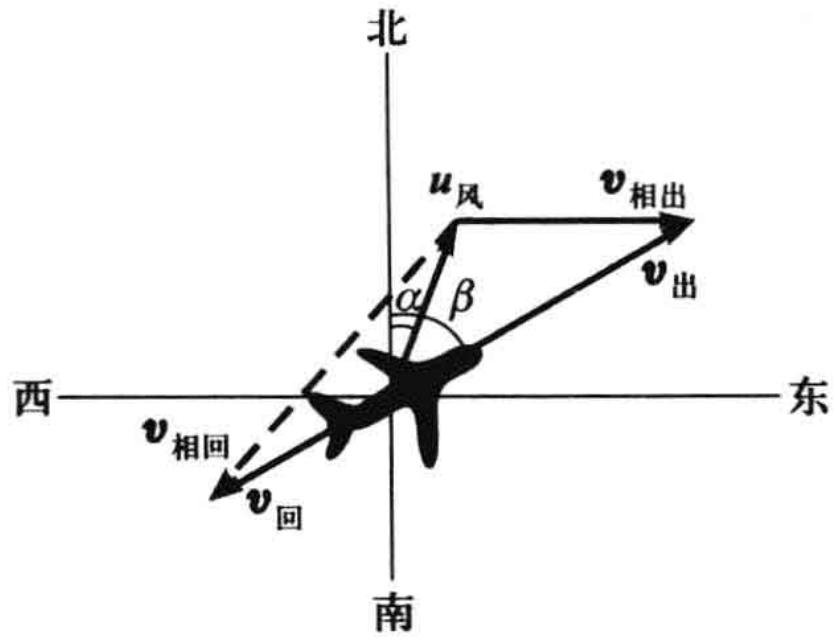
\includegraphics[width=0.4\textwidth]{figures/fig1-29.jpg}
  \end{figure}

\vfill
\newpage